\section{Social Weaver - Concrete Domain Level}\label{sowe-concrete}

\subsection{Social Weaver - Firefox Plugin} \label{sowe-firefox}
This section will briefly explain what technologies we use for firefox plugin development and describe in detail how the Social Weaver plugin is implemented.

\subsection*{Firefox}
Firefox is a free web browser that has been released 2004 by the Mozilla Foundation\footnote{\url{www.mozilla.org}}. It is being multi-licensed under Mozilla Public License (MPL)\footnote{\url{http://www.mozilla.org/MPL/1.1/}}, GNU Lesser General Public License and GNU (LGPL)\footnote{\url{http://www.gnu.org/licenses/lgpl-3.0.de.html}} General Public License (GPL) \footnote{\url{http://www.gnu.org/licenses/gpl-3.0.html}}. 

The reasons why we chose Firefox as prototype environment are the high distribution of the browser and an easy extendability with plugins, extensions and so on.

\subsection*{Firefox Plugin Development}
To improve readability of the coming section \ref{firefox_plugin_requirements} \nameref{firefox_plugin_requirements}, we will discuss some aspects from the Mozilla Add-on SDK (Version 1.13) \footnote{\url{https://addons.mozilla.org/en-US/developers/docs/sdk/latest}}. Readers who are not interested to much into technical detail or are familiar with the technologies can skip this section.

The used methods will not be just explained independtly but brought into context to our prototype planning so it becomes clear what purpose they have. 

The Add-on SDK allows to create add-ons for the browser using the most common web technologies (like HTML, CSS, JavaScript, ...). Furthermore it provides a Low-Level-API and a High-Level-API set. The most important interfaces that are being used for our prototype are High-Level-Interfaces and will be explained in the following.

\begin{description}
\item Panel\\
A \emph{panel}\footnote{\url{https://addons.mozilla.org/en-US/developers/docs/sdk/latest/modules/sdk/panel.html}} is very flexible dialog window. Its appearance and behavior is specified by a combination of a HTML and a JavaScript file. Additionally a CSS file might be used to change the look even further. The limitations of a panel are the limitations of the mentioned technologies. 
A panel is meant to be visible temporary and they are easy to dismiss because any user interaction outside the 

\begin{figure}\centering
		
\includegraphics[width=8cm]{images/example-panel.png}
		\caption{An example for a \emph{panel} that shows a list of anntations}
		\label{example-panel}
\end{figure} 

We will use the \emph{panel} for getting user input, displaying information (like in screenshot \ref{example-panel}) and to integrate our social media web elements. 

Actually the flexibility of \emph{panel} is the reason why our prototype is able to support social weaving for basically any web element that can be represent in HTML code. Still it is necessary to embbed the external HTML code which may leads to boundaries and difficulties.

\item Simple-Storage\\
This module\footnote{\url{https://addons.mozilla.org/en-US/developers/docs/sdk/latest/modules/sdk/simple-storage.html}} is an easy to use method to store basic properties (booleans, numbers, strings, arrays, ...) across browser restarts. 

With an operation like

\begin{lstlisting}
var ss = require("sdk/simple-storage");
ss.storage.myNumber = 41.99;
\end{lstlisting}

we store a number like an object and can it access just as easy like that. The price for such a simple usage is paid with high limitations. For instance searching is basically not possible. Nevertheless we can store an array and search the array. 

That is exactly the way how we store our annotations for our prototype. More details will be provided in the next section.

\item Page-Mod\\
The \emph{page-mod}\footnote{\url{https://addons.mozilla.org/en-US/developers/docs/sdk/latest/modules/sdk/page-mod.html}} module enables us to act in a specific context related to a web page. Then it becomes possible to attach JavaScripts to it and to parse or modify certain web page parts.

In our context we are going to use \emph{page-mod} to parse the HTML code to find elements that can server as anchors for annotations. And of course to find elements that are already annotated.

\item Widget\\
The module that is called \emph{widget} \footnote{\url{https://addons.mozilla.org/en-US/developers/docs/sdk/latest/modules/sdk/widget.html}} is simply an interface to the Firefox add-on bar\footnote{\url{https://developer.mozilla.org/en-US/docs/The_add-on_bar}}. It is possible to attach \emph{panels} and trigger operations by clicking the \emph{widget}. 

\begin{figure}[h!] \centering
		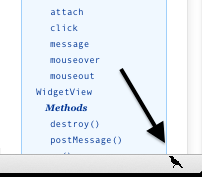
\includegraphics[width=7cm]{images/example-widget.png}
		\caption{Example for a widget serving as activation button}
		\label{example-widget}
\end{figure} 

We will use a widget to switch between different modes (see coming section \ref{display-management-requirement} for more details about how the mode-system works).

\item Self\\
\emph{Self}\footnote{\url{https://addons.mozilla.org/en-US/developers/docs/sdk/latest/modules/sdk/self.html}} provides access to add-on specific information like the Program ID\footnote{\url{https://addons.mozilla.org/en-US/developers/docs/sdk/latest/dev-guide/guides/program-id.html}}, which is important for an official distribution of the add-on. More meta information like the name or the version are accessible via the \emph{self} module. Also bundled external files are integrated by \emph{self}.

Even though it is an important module and part of the plugin - there is no specfic usage relation to the system we use. 

\item Notifications\\
This module\footnote{\url{https://addons.mozilla.org/en-US/developers/docs/sdk/latest/modules/sdk/notifications.html}} displays toaster\footnote{Toasters are commonly called notifications that just appear, or slides in the users view - like a toast hops up.}-messages\footnote{\url{http://en.wikipedia.org/wiki/Toast_(computing)}} that disappear after a short time.

We use these to keep the user informed without bothering him to much by forcing him to dismiss trivial notifications.

\item Request\\
This simple to use but yet powerful module \emph{request}\footnote{\url{https://addons.mozilla.org/en-US/developers/docs/sdk/latest/modules/sdk/request.html}}, lets us perform network requests. Once we create a \emph{Request} object we can specify whether it is a GET, PUT or POST request. These request types are specified by the REST standard so any web service that supports REST is able to interact with this module\cite{fielding2000principled}. The response from a server is directly accessible like any other JavaScript object. 

We are going to use \emph{request} for our communication with our synchronization web service. This includes sending updates, made with the plugin instance, to the server and receiving updates, that were made in other sessions or with differen plugin instances, from the server. 

\end{description}

\subsubsection*{JQuery}
\emph{jQuery}\footnote{\url{http://jquery.com/}} is a free JavaScript library under the MIT License\footnote{\url{http://www.mit.edu/}} that offers many functions for modifying DOM trees. It has been released 2006 in context of a BarCamp\footnote{\url{http://en.wikipedia.org/wiki/BarCamp}} in New York.

Even though this library is not a part of the Mozilla Add-on SDK it is being heavily used by it. Basically any operation that changes or traverses the HTML code (like changing the background color of web elements) is being reached with jQuery.

The reason why jQuery makes it so easy to handle operations on HTML code is based on the selector that searches the DOM tree. Most jQuery operations are based on elements in the DOM tree. With the selector \verb+jQuery()+ (which can be equally written as \verb+$()+) any element in the DOM tree can be used to create a jQuery object. This object can be used to perform modifiying operations on it. For instance lets step through the following short operation:
\begin{lstlisting}[language=JavaScript, numbers=left]
$('.user-name').click(function(){
   this.empty();
});
\end{lstlisting}

In line one we use the \verb+$+ selector to find any element in the DOM tree that has the id \verb+user-name+. Since we use the jQuery selector, any found element can be handled as a jQuery object. This way \verb+click(function(){...})+ appends a click observer to all elements. Any time one of those elements is clicked by the usert, this triggers the function. This function inlcudes \verb+this.empty()+ that will only remove all content inside the element. 

Another and more related example of jQuery usage is used in the selection part of the plugin:
\begin{lstlisting}[language=JavaScript, numbers=left]
$(":visible").filter(function(index) {
  if(this.content()){
      return true;
  }else{
      return false;
  }
}).mouseenter(function() {...}
\end{lstlisting} 

First of all we request all elements that are visible to the user by using \verb+$(":visible")+. Because it is unlikely that a user will try to select an element without any content - we filter all elements from the result set that are empty. (Such elements can be placeholders, flexible empty space and so on.) Now that our results contains mostly relevant elements to the user, we append \verb+.mouseenter()+ to recognize when the curser is placed above the element. The skipped function itself contains operations to recognize more user operations and element analysis. To discuss more code in detail would be beyond the frame. 

We only have seen a brief overview about jQuery operations. To fully understand how the prototype works and to operate with the script support it is adviced to gather a better overview using for instance the official W3 introductions: \url{http://www.w3schools.com/jquery/}. 

\newpage
\subsection{Requirements for the Plugin}\label{firefox_plugin_requirements}
Let us recap what requirements we gathered in section \ref{browser_plugin} on the abstract domain level \cite{van2009requirements}:

\begin{enumerate}
\item Displaying and managing a comment box related to specific web elements
\item Managing several comment boxes without disturbing the view on original content
\item Communication to server application
\item Creating Anchors
\item Creating content in uniform sending format
\item Parsing content from uniform sending format
\item Identifying web elements across different user sessions
\end{enumerate}

In the following concretization we apply the abstract requirements to our environment which is the \emph{Mozilla Plugin Development SDK} \footnote{\url{https://addons.mozilla.org}}. In the following we will handle each and every requirement, mentioned above, seperately:

\subsubsection{Display Management Requirement}\label{display-management-requirement}
Obviously "Displaying and managing a comment box related to specific web elements" consists of multiple sub requirement that we need to distinguish. 

\begin{figure}\centering
		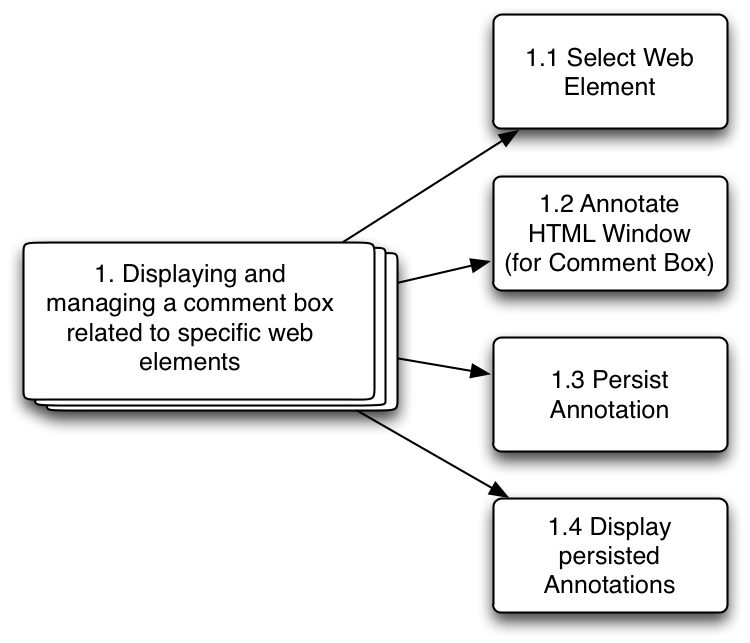
\includegraphics[width=10cm]{images/abstract2concrete-1.png}
		\caption{Partition of the first plugin requirement to sub requirements}
		\label{abstract2concrete-1}
\end{figure} 

Before we are able to annotate something, we first of all need a function to select or recognize a web element the users cursor points to (check 1.1 in figure \ref{abstract2concrete-1}). \emph{Selecting} in this context means that we analyze the Document Object Model (DOM)\footnote{\url{http://www.w3.org/DOM/}} tree. The selection itself is easy to implement using the function \emph{mouseenter} and \emph{on('click')} from jQuery library\footnote{\url{http://jquery.com/}}. It becomes problematic to find this element again without any user interaction. Therefore we need to set well chosen parameters that are used to determine the element. Next time we need to find the element - only the parameters can be used to finde the element in the DOM tree. This issue will be topic in the section \ref{sowe-script-support} \nameref{sowe-script-support}.

Theoritically it could be possible for user to select any element in the web view - but practically this would make the selection procedure confusing for development as well as for the user. Therefore we apply some filters. Elements like empty boxes, placeholders and so on will not be selectable. 
But still it should be clear to the user what he might select. 

To achieve this functionality we create thin rectangles around every element that is an selection option. These rectangles only appear for time the plugin is in selection-mode and uglify the web view just for a certain time. More on the different mode types in \ref{user-disturbance} \nameref{user-disturbance} .

Now that we can locate a specific web element we may annotate some social web element. For reasons of flexibility and simplicity we just annotate a HTML window (check 1.2 in figure \ref{abstract2concrete-1}), where we can inject any external HTML code. The Mozilla SDK high-level APIs \footnote{\url{https://addons.mozilla.org/en-US/developers/docs/sdk/latest/modules/high-level-modules.html}} offers all necessary tools to insert a HTML box as a \emph{Panel}\footnote{\url{https://addons.mozilla.org/en-US/developers/docs/sdk/latest/modules/sdk/panel.html}}.

The annotation anchors will be visible to the user in form of a colored background that we create by modifying the DOM tree.
If the user clicks on such an element the already existing panel will be opened. 

\begin{figure} \centering
		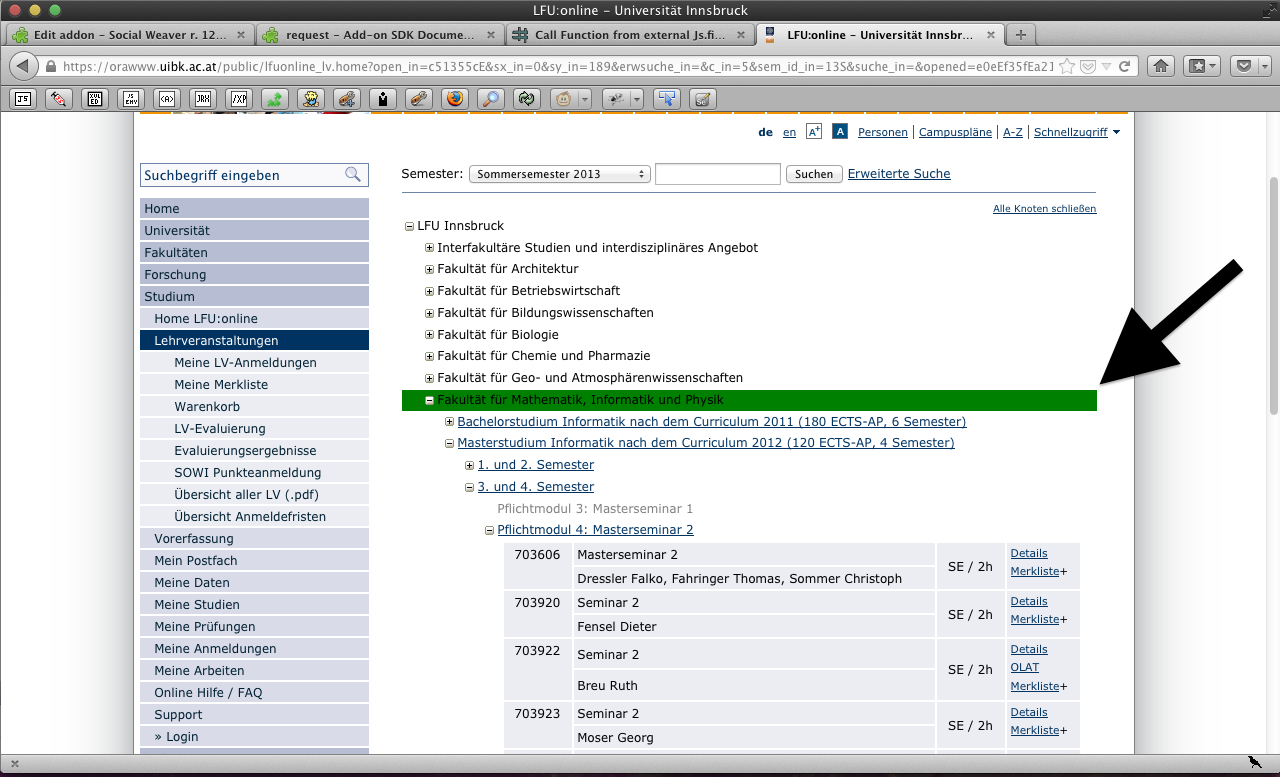
\includegraphics[width=13cm]{images/annotation-rectangle-sample.png}
		\caption{Rectangle shows that the underlying element is possible for annotation}
		\label{annotation-rectangle-sample}
\end{figure} 

To decouple our annotated data (like anchors, annotations, ...) from the actual synchronization, which will be covered later, we want to use a storing system that is also provided by the Mozilla SDK (see 1.3 in figure \ref{abstract2concrete-1}). The high level API \emph{simple-storage} \footnote{\url{https://addons.mozilla.org/en-US/developers/docs/sdk/latest/modules/sdk/simple-storage.html}} enables us to store all information we need and recall them. Just the synchronization mechanism should modify this data set. All displaying procedures should be outside of server communication reach. This means that if an annotation is created, the changes are written locally into the plugin local data storage. And only after the persistence is complete, the synchronization procedure will be initiated. While synchronizing the changes will be transmitted to the server. 

The last sub requirement is to redisplay existing annotations (check 1.4 in figure \ref{abstract2concrete-1}) from our \emph{simple-storage}. Besides using the same techniques for drawing content and retrieving it from the storage we need to match the web page content to our saved annotations. For that we use a matcher instance that checks the DOM tree for IDs that we are already using. 

This is actually only trivial on a very simple basis. Let us assume that we will have more than one element attached to the same web element. Or we have different user sessions and/or include a workflow so that we need to distinguish the same element for different instances of the webpage. Than it becomes quite complicated to generate IDs that we can rely on. Nevertheless these issues will just affect the way we assign IDs to elements and how we retrieve them. The requirement 1.4 is just about matching existing IDs to a web page. 

As already mentioned we use a matcher that checks the DOM tree for IDs. In case we have an anchor in our \emph{simple storage} then we modify the web page HTML code similar as we did for requirement 1.1. Visual differences are that we do not modify the background of an element but generate an rectangle around it instead (see screenshot \ref{annotation-rectangle-sample2}). 

\begin{figure} \centering
		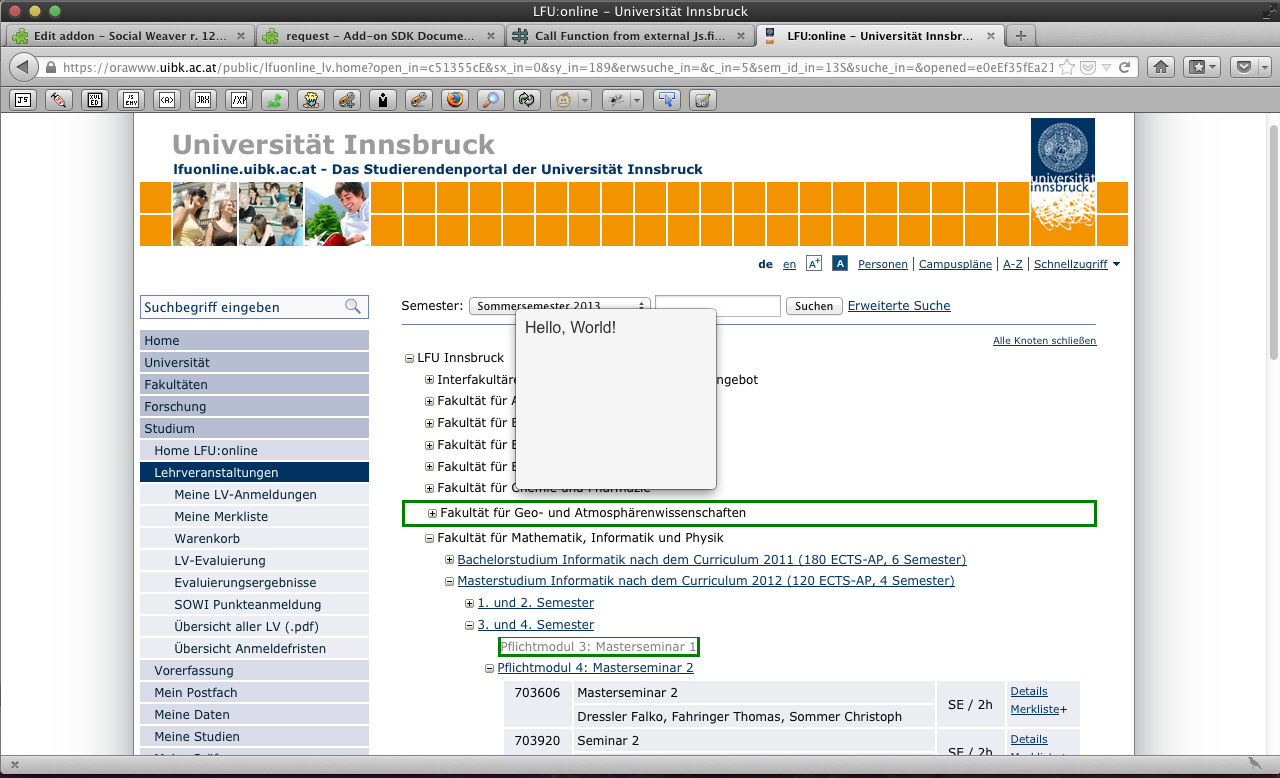
\includegraphics[width=12cm]{images/annotation-rectangle-sample2.png}
		\caption{Rectangle shows that the underlying element is possible for annotation}
		\label{annotation-rectangle-sample2}
\end{figure} 

This way we are able to show the user which elements are annotated. Of course without further information it is not obvious what is annotated exactly. What we need is a easy to access functionality so that the user can find out what the annotation is. 

For that reason we modify the above mentioned matcher class to generate a panel in case the user performs a \emph{mouseenter} operation. This panel should show a brief version of the attached social element. In our case it could be the name of the context the comment box is related or the names of the attendees (our example screenshot just print outs "Hello, World!" \ref{annotation-rectangle-sample2}). 

\subsubsection{Managing several comment boxes without disturbing the view on original content}\label{user-disturbance}

This requirement is not directly about functionality but should ensure a positive user experience. It will be possible to attach annotations to nearly any element in a web application. This is a lot of potential additional footage. Nevertheless the user needs to be in the position to navigate like usually within the application. 

Basically there are two options to guarantee such a requisition. Either we minimize the overhead that we display into the web view or we display additional information only at the appropriate time. To achieve the best results we combine both possibilities by introducing the mode system:

The plugin will have several modes that support different functionality and show different content. Those modes can be switched by clicking the widget in the addon bar. Every mode has its own logo, see Figure \ref{mode-logos}. 

\begin{figure}[h!] \centering
		
\includegraphics[width=13cm]{images/mode-logos.png}
		\caption{Widget representation for different modes}
		\label{mode-logos}
\end{figure} 

We distinguish the following modes:
\begin{enumerate}
\item Default mode \\

In the default mode the plugin runs passively. It does not disturbs the user but runs synchronization and matching procedures in background. When the user opens a new web view, the plugin checks its database for annotations that belong to the view. If a positive match is found, it will be drawn into the users webview. 

The navigation of the browser is as usual, except for the annotations that include a click handler that triggers the function for opening the social element.

\item Selection mode \\ 

The selection mode interferes eminently with the navigation and the representation of the regular browser view. Activating the selection mode will mark all selectable elements with rectangles around it. Moving the cursor around the web view will additionally mark the element beneath the cursor to visualize what element will be marked when clicked. 
In this  mode clicking links, buttons and so on, will not trigger the functionality of those elements but instead select them so an annotation might be created. 

Disabling the selection mode will clear the view from the previously mentioned marks. Only successfully created annotations will remain persistent. 

\item Deactivated mode \\ 

Deactivating the plugin entirely disabled any functionality. This can be useful in worst cases like that the plugin prohibits regular navigation or the annotation marks interfere with the users view.
\end{enumerate}

The mode system could be a starting point for extending Social Weaver for multiple user sessions in one plugin context. Or providing securely authenticated sessions that can only be activated when correct credentials are provided. 

\subsubsection{Communication to server application}
To share our comments or annotations with other users we will need a server side synchronization procedure. This section is only about the requirements that are related to the plugin side. (Details to the server side will be discussed in \nameref{server} \ref{server}.)

The first step to achieve this goal is to establish a communication between the plugin and a web service. For this purpose we are going to make use of the \emph{request} module from the Mozilla Add-on SDK. It provides an easy to use JSON\footnote{\url{http://www.json.org/}} and REST(\cite{fielding2000principled}) assistance. 

We split this into the following sub requirements:
\begin{description}
\item Plugin receives updates from server\\
What the plugin needs to know from the server is a set of Anchors. Those Anchors contain information like the author identification, a timestamp and of course the content.
(see \ref{creating_triplets}) 
So at this point we assume that our server will provide a set formatted in JSON. The plugin generates a request to retrieve this data. 
\begin{figure}
\begin{lstlisting}[language=JavaScript]
var sync = Request({
      url: 'http://localhost:9998/anchor',
      onComplete: function(response) {
        for(var i = 0; i<response.json.length; i++){
            var r = response.json[i];

            newAnchor = new Array(r.anchorURL, 
		r.ancestorId, r.anchorText);
            var newAnnotationText = r.annotationText;
            handleNewAnnotation(newAnnotationText, 
		newAnchor);
     };
   }
});
sync.get();
\end{lstlisting}
\label{anchor_sample_code}
\caption{Sample JavaScript code for retrieving JSON objects from a web service with a GET REST request}
\end{figure}

This goal is surprisingly simple to achieve. In the sample code \ref{anchor_sample_code} we just need to specify the URL of the web service and we are able to access the JSON objects right away exactly like JavaScript objects. Then we use the JSON objects to create an anchor entity and use the existing \verb| handleNewAnnotion(newAnnotationText, newAnchor)| method to store it in our \emph{simple-storage} list. 

Our prototype is a proof-by-concept system, therefore we keep the synchronization really simple. Instead of checking for new annotations and match them with the already existing data, we just rewrite our local plugin data set with a copy from the server. This technique could easily lead to corrupt and inconsistent data sets. But since the prototype is not meant to be used for confidential data or in any real world scenario at all - we will just take our risks.

\item Plugin sends updates to server\\
When a user creates a new annotation or modifies it - the plugin should send an update to the web service immediately. Again we will set up a method using the \emph{request} module. 
\end{description}

How the data format looks like and how we will parse incoming messages will be reviewed later (in the sections \ref{creating_triplets}, \ref{creating_content} and \ref{parsing_content}.)

\newpage
\subsection{Social Weaver - Web Service}
The coming part will be about the implementation of the web service that provides interfaces for our previously built plugin.

\subsection{Used Technologies}
Before we disucuss our web service architecture we first of all will list the used technologies and give a brief explanation. Readers who are farmiliar with the following terms may skip this section. 
After pointing out the architecture, we will map our defined requirements to our implementation and explain how those are achieved.

\begin{description}
	\item Model View Controller (MVC)
	\item OpenJPA
	\item PostgreSQL
	\item RESTful Web Services
	\item Spring
	\item AspectJ
\end{description}

\subsection{Web Service Architecture}
The web service is a common MVC architecture that uses JSON/RESTful interfaces. The persistence layer is connected to a PostgreSQL database using OpenJPA. 

Our main entities are the anchor and social element. The anchor has been already discussed from the concept point of view. The entity contains all the parameters that are necessary for matching web elements. This set of parameters can differ from one web application to another. Additionally the anchor entity contains an unique object identifier (OID) that defines the anchor even across different user sessions. This way updates can be performed more easily without having to check for all parameters every time. Which would be hard especially in those cases where an unusual set of matching parameters is being used. To avoid this difficulty but to still keep all parameters related we generate a hash from a combination of all relevant parameters. This hash is used as OID. 
Besides that the Anchor holds a timestamp with information about the last modified date. We use this data for the synchronization procedure. 

The social element entity is handled as a separate entity but from the concept persepective it is a part of the Anchor. Basically it works as a container for any kind of social content. Because our prototype will just provide a simple HTML inject, the SocialElement will contain an URL and a reference to the Anchor. But it will be extendable to hold data for native and more complex social element types. 

The entities are implemented as beans and therefore being directly persisted in the PostgreSQL database.

According to the model view controller pattern there are also controllers for the entities that provides several interfaces that are accessible through the standard REST requests. 

\begin{figure}[h!] \centering
		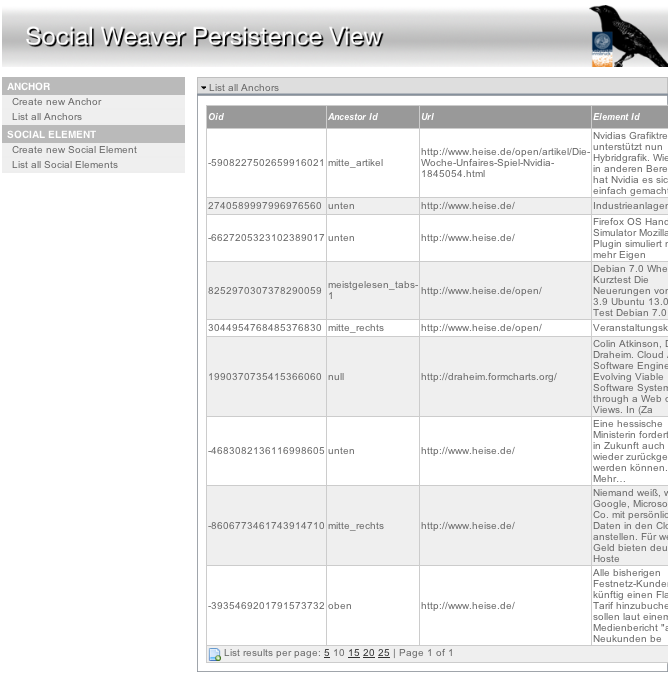
\includegraphics[width=9cm]{images/sowe-mvc-view-screenshot.png}
		\caption{Screenshot from Social Weaver Persistence Web View}
		\label{sowe-mvc-view-screenshot}
\end{figure} 

The View from our Model View Controller architecture is a web view that allows the user to check the content manually (see Figure \ref{sowe-mvc-view-screenshot}). This is just a pleasent side feature and not related to our Social Weaving use cases and for that reason this part should be discussed no further.


\subsection{Requirements for the Web Service}
In section \ref{Social Weaver - Server Application} we defined the following requirements for the web service:

\begin{enumerate}
	\item Offer service that receives messages from plugin-clients
	\item Synchronization for requests from different user-session
	\item Persist updates into a database
	\item Keep the server application independent to weaved-into web application
	\item Parse incoming messages
	\item Create outgoing messages
\end{enumerate}

\subsubsection{Offer service that receives messages from plugin-clients}
Cleary we accomplish this requirement with the RESTful web service interfaces. The messages that we transmit are the Anchor information right away. 


\subsubsection{Synchronization for requests from different user-session}

\subsubsection{Persist updates into a database}

\subsubsection{Keep the server application independent to weaved-into web application}

\subsubsection{Parse incoming messages}

\subsubsection{Create outgoing messages}

\newpage
\subsection{Social Weaver - Script Support}\label{sowe-script-support}
The following part will explain how the script support looks like in detail for our firefox plugin. In section \ref{abstract-script-support-reqs} we learned about the purpose of the script support and what its goals are. The coming part will apply this knowledge practically to the prototype development. Before we start stepping through the gathered requirements from \ref{abstract-script-support-reqs}, a brief example of a script use case will be explained to provide a better overview to the reader.

A script contains the information about how an element in a web view might be found. We use JSON as format for the scripts because of the support that JavaScript provides for that standard. The script defines a set of rules that will be used to perform operations on the selected element. The results from these operations will be generated to a payload. This payload might be the information for anchors, URL and content related to social elements. The server handles this payload as one value and does not parse it. All meta information that are needed by the server will be transmitted separately from it. To understand how the script is used to generate an anchor format take a look at the example:

\begin{lstlisting}
{
    rules:
    [

         {"doc_location" : "document.location.toString()"},
         {"element_content" : "$(matchedElement).text()"},
         {"element_children" : "$(matchedElement).children().text()"},
         {"element_content": "matchedElement.innerHTML"},
         {"dom_path": "true"}	
    ]
}
\end{lstlisting}

The purpose of this script example is to show the different possibilities and not a real scenario use case. It will become obvious why this set of parameters would be no good choice. 

Basically a script is a set of rules. A rule consists of a keyname and the actual operation that is being used to perform an action. The keyname can be any string withing quotes chosen by the script author. The keynames should be unique in one script though. The operation part offers different opportunities:

\begin{itemize}
	\item jQuery Operation \\ 
	jQuery is a great possiblity to traverse the DOM tree and it is possible to inject jQuery commands directly in the script. It is necessary that the command returns a string that is used for identfitication. The first line
		\begin{lstlisting}
		         {"doc_location" : "document.location.toString()"}
		\end{lstlisting}
	would tell the plugin to save the document location - which is the plain URL in most cases. 
	
	To trigger an operation related to the element that has been clicked by the user we might use the keyword \verb^matchedElement^. In case a jQuery method is used it is still necessary to transform the matched element to jQuery format (\verb^matchedElement^ $\rightarrow$ \verb^$(matchedElement)^). 
	
	\item	 JavaScript Operation \\
	Even though most functionality related to DOM tree traversing should be covered with jQuery it might be of use sometimes to use JavaScript commands directly. 
		\begin{lstlisting}
		         {"element_content": "matchedElement.innerHTML"}
		\end{lstlisting}
	This line is an example for how to retrieve the HTML content of an element. This information might be used for matching elements for instance. 
	
	\item Predefined Operation \label{predefined-operation}
	Some functions we need are not directly provided using JavaScript. The best example for such a case is the DOM tree path. We can use the DOM tree path for distinguishing similar elements. This functionality is provided by the plugin and can be enabled or disabled with the rule:
		\begin{lstlisting}
		         {"dom_path": "true"}
		\end{lstlisting}	
\end{itemize}

\subsection{Requirements for the Script Support}

In the abstract section (\ref{abstract-script-support-reqs}) we defined a couple of abstract requirements that we need to specify for a proper implementation. Those requirements were:

\begin{enumerate}
	\item Container of all necessary information for element matching
	\item Decoupled from browser plugin and server backend
	\item Syntax that is easy to read and write
	\item Extension of the plugin with parsing methods
	\item Default matching procedure should be provided (so the overall functionality is not limited when no scripts exist)
	\item Scripts should be related to a single or a set of URLs
\end{enumerate}

\subsubsection{Container of all necessary information for element matching}

For matching different elements we need the flexibility to use a variable set of rules. It would be a drawback to have a static rule system. The problem is that in some web views we need different operations to match elements than on others. Depending on the environment we need a specific container with the rule set. 

We solve this issue by introducing the payload container that contains a JSON array with all information that is set by the script. This way we are able to extend information for element matching and modify it just by changing the script. The plugin and backbone of our system will not necessarily have to be changed because it will always be handled as a single JSON string.

\subsubsection{Decoupled from browser plugin and server backend}\label{decoupled-req}

The script itself does not contain any information of the browser plugin type or the server module. The defined rules need to be supported by the plugin though. 

A plugin that does not support jQuery commands would not work with our script example from above. Or the \emph{predefined operation} (mentioned in \ref{predefined-operation}) is another case that needs to be supported by the plugin. Using unknown or unsupported operations will lead to unexcpected results.  

The server on the other hand is completely decoupled from the script support. The payload is just one column and the information about element anchors is of no use for the server. This is way the payload will not be parsed on the server. 

Even corrupt payloads that cannot be used by the plugin will be perfectly synchronized at the back end. This might seem not much of use at first appearance. But there is the case when a the payload for matching an element becomes defect not by using wrong rules, but because of some changes in the web view. Then we still want to keep the information about the element and just re-create the payload to it. Hence it makes sense to keep even those elements in the server database.

\subsubsection{Syntax that is easy to read and write}

It is a desirable goal for the future to have a system, like a script generator, that can be used be persons without any technical knowledge. But since we conduct prototype development we will at least assume knowledge about web development. To choose the right rules and operations for element matching, requires this kind of knowledge anyway. 

JSON is commonly used format and even possible to read by persons without technical knowledge. When providing a template with some example rules it is obvious to see how these rules might be extended. 
The most challenging part is to find and define the correct set of rules - but this is beyond the scope. 

Beyond the criterion that scripts are human readable it would be easy to create a form or generator with a graphical interface to generate such scripts. Error handling could be supported already at this point. Even more desirable is an automatic script generator that generates scripts from user behavior without his active interaction (or at least minimal). 

\subsubsection{Extension of the plugin with parsing methods}

When we were talking about rules and operations for element matching, this included short Java Script or jQuery commands. Technically we are not limited to short commands and it is possible to insert a whole command block as a rule. But for debugging reasons this is not a good solution. And some operations may require more than just a chain of jQuery commands. 

For example lets take the procedure of determining the DOM path of an element in the tree. The idea is to start with the class name of the element itself. Then check the class name of its parents so long until the root of the DOM tree is reached. All names chained together describe the path of the element in the tree. The fact that this result is not necessarily unique underlies the problem that DOM trees are often ambigious. We will take a closer look on this issue in \ref{ambiguity-problem} \nameref{ambiguity-problem}. But for some web views the DOM path still might be the right choice. 

To understand why such a procedure is not possible to be fitted in a script we need to take a look at the code first:

\begin{lstlisting}[language=JavaScript]
    var rightArrowParents = [];

    $(this).parents().not('html').each(function() {
        var entry = this.tagName.toLowerCase();

        if (this.className) {
            entry += "." + this.className.replace(/ /g, '.');
        }

        rightArrowParents.push(entry);
    });
    rightArrowParents.reverse();    
    var domPath = rightArrowParents.join(";");
\end{lstlisting}

In line three we initiate a loop for all parent elements of the selected element \verb^this^. We watch out for every parent that has a \verb^className^ in line six. In a positive case we add this information to our path result. 

The problem why we cannot insert such an operation into a script is, that we need an outside variable for keeping track of the results through the loop iterations. Line three until eleven is the actual jQuery command. But it would be a mess to pass the whole code with the script. Theoretically it would be possible to support such scripts but it would make the script idea even more error prone. 

Instead we use \emph{predefined functions}. Those functions are implemented directly in the plugin and can be triggered using defined rules in the script. 

To enable the DOM path parameter in the rule set we would just need to insert this rule:
\begin{lstlisting}
         {"dom_path": "true"}
\end{lstlisting}
The plugin would recognize this rule and run the code that determines the DOM path. In the section \ref{decoupled-req} we already mentioned that this way of supporting more complex operations leads to minor coupling between plugin and script. 

\subsubsection{Default matching procedure should be provided} \label{default-matching-procedure}

Even though it is not possible to provide a default matching algorithm that will apply to any web view, it is desirable to at least have some default matching in case to specific script for the visited URL exists. If the user visits an new environment there is at least the chance that some elements might be matched.

To fullfill this requirement the plugin will provide a default script. When a new web view will be loaded - all scripts will be checked whether one of them applies to the new page. If it is not the case the default script will be chosen and the user notified. 

\subsubsection{Scripts should be related to a single or a set of URLs}

Every script, except for the default script from \ref{default-matching-procedure}, mostly needs to be related to a specific environment. When we talk about environment in this case, it means views that inherit from a root URL. As example a script can be related to \url{http://www.gnu.org}. But any page that has this URL as root, like for instance \url{http://www.gnu.org/philosophy/philosophy.html}, will still apply to the same script. 

The assumption is that views in the same environment apply to the same web architecture and hence its elements can be identified similarly. 

Obviously this must not hold for every case. Theoretically a web view can has a totally different architecture than its root. But for prototype development this drawback is considered as tolerable. 

\newpage
\subsection{Ambiguity Problem}\label{ambiguity-problem}

Throughout the abstract (\ref{sowe-abstract}) and concrete (\ref{sowe-concrete}) section about the prototype development we often noticed issues that make it tricky to achieve the proposed goals. The greatest challenge by far is the unique recognition of elements in a web view. More precisely: the finding of an element in the DOM tree. 

This procedure consists of the two steps:
\begin{enumerate}
	\item User choses element from view
	\item Plugin searches for this element from the DOM tree
\end{enumerate}

The first step is easy because we have the clear information from the user input. The hard work is done by the user. Still our problematic situation takes place already at this point. 

Hence the plugin needs to know in what way it is going to identify the element in the second step, it is necessary to gather all the information in first step. This is were the rules from a script (\ref{sowe-script-support}) come in. Those rules are commands that are executed and retrieve results. Those results identify the element. 

In the second step, when a view is opened, all appearing elements are checked with the script rules and the results compared to our results from step one. If the results appears to be the same - we assume it is the searched element. 

The fact that we can only assume, finally leads us to the actual problem of this section. The DOM tree can be ambiguous and as a matter of fact this is no exception.

\subsubsection{Ambiguous Grammar}
\begin{figure}[h!] \centering
		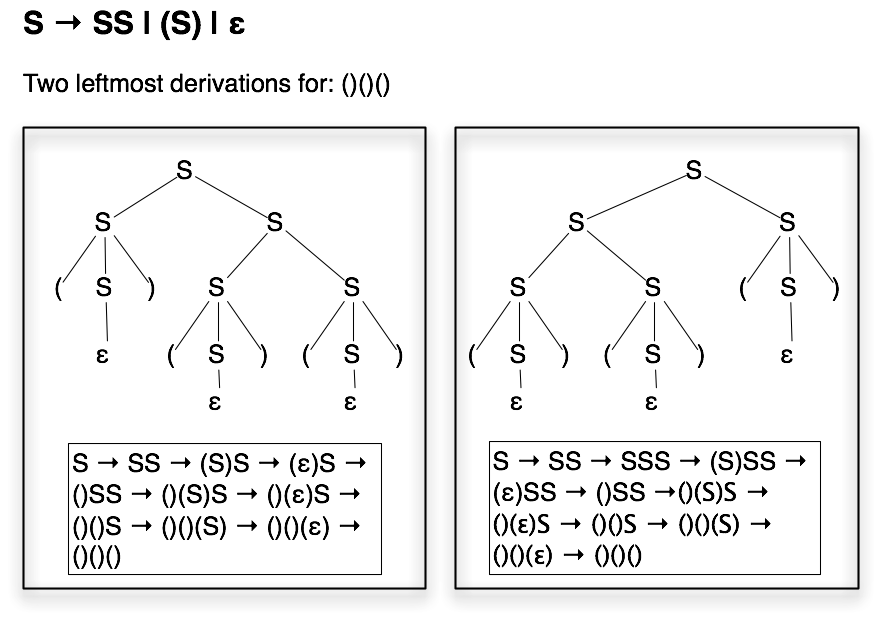
\includegraphics[width=11cm]{images/ambiguous-grammar.png}
		\caption{Example for an ambiguous grammar}
		\label{ambiguous-grammar-pic}
\end{figure} 

We know the origin of ambiguity in computer science from formal grammars. A grammer is ambiguous for which there exists a string that has more than one leftmost derivation. Check Figure \ref{ambiguous-grammar-pic} for a common example of a ambiguous grammar.
\begin{lstlisting}[mathescape]
S $\rightarrow$ SS | (S) | $\epsilon$
\end{lstlisting}
This generates a chain of correct opening and closing brackets. The grammar is ambiguous because we have to ways of generating the same string \verb^()()()^. For the parse tree and step by step creation see again the figure \ref{ambiguous-grammar-pic}.

\subsubsection{Ambiguity for Element Matching}

What is the concern of ambiguous grammars when we talk about web architectures? We will use the basic idea of ambiguity to describe the problem giving elements unique parameters. Imagine we would try to identify elements just on their location in the DOM tree. At a first glance this may appear as an effective way since we are used to storing data in tree based data structures. 

We explain the problem with the HTML example in Figure ...
\begin{figure}
\begin{lstlisting}
<html>
	<head>
			<title>Software Development</title>
	</head>
	<body>
		<b>Software Development Activities</b>
		<ul>		
			<li> Requirements 
			<li> Construction 
			<li> Deploying		
		</ul>
		<b>Software Development Methodologies</b>
		<ul>		
			<li> Spiral
			<li> V-Model 
			<li> Scrum		
		</ul>
	</body>
</html>
\end{lstlisting}
\label{dom-html-example}
\caption{HTML example for showing ambiguity}
\end{figure}


\begin{figure}[h!] \centering
		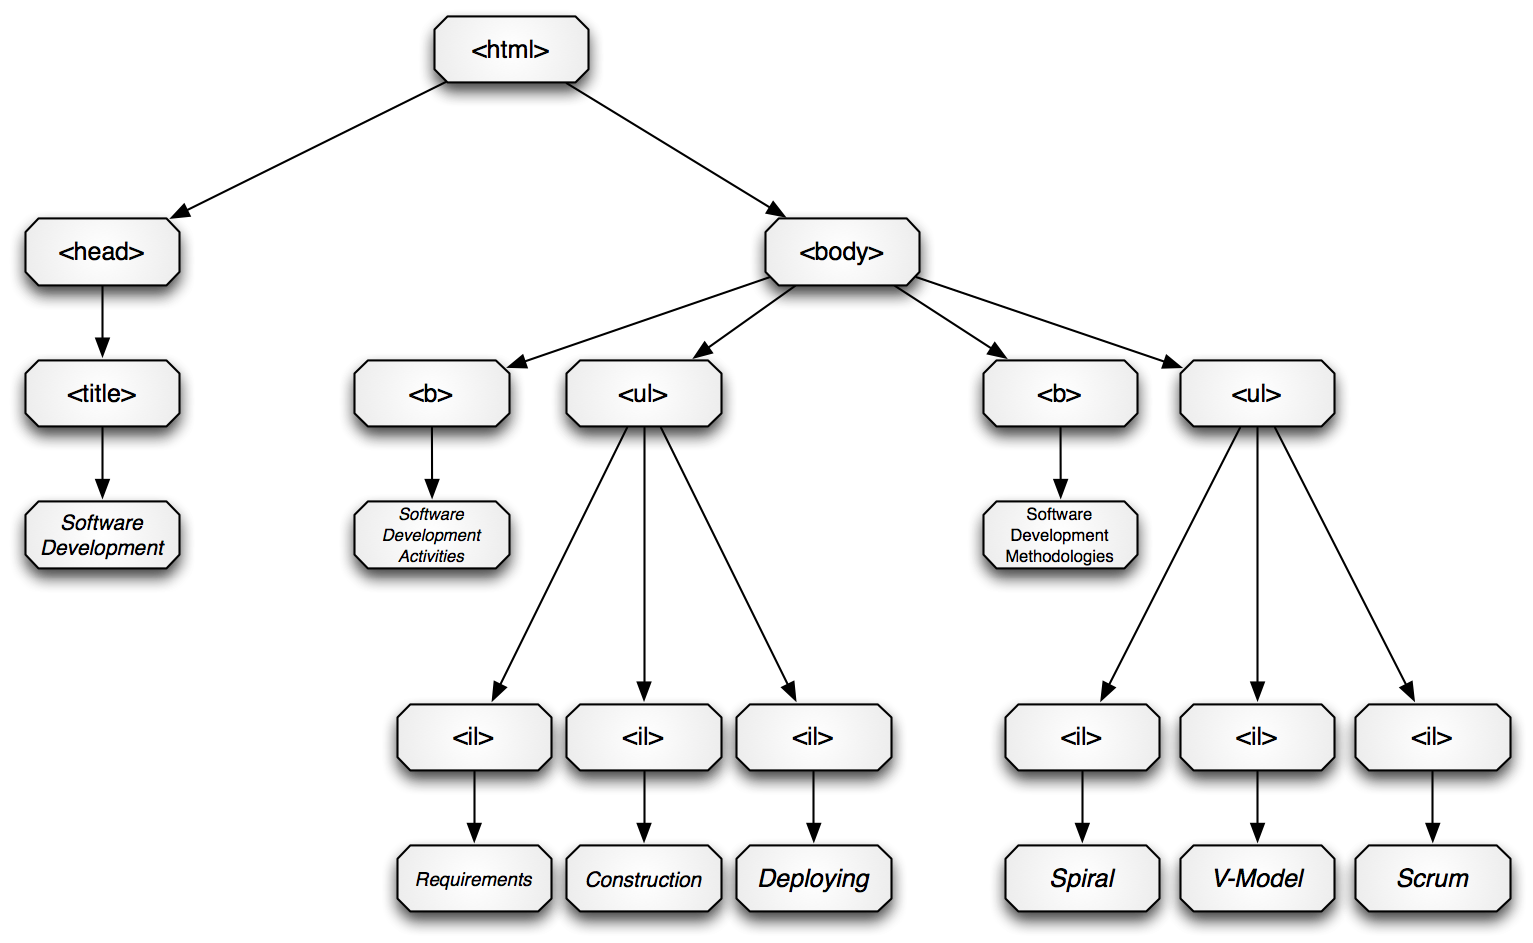
\includegraphics[width=13cm]{images/dom-tree-example.png}
		\caption{DOM tree represenation for HTML code in Figure \ref{dom-html-example}}
		\label{dom-tree-example}
\end{figure} 

Determining the DOM path for \verb^Software Development^ would return the value: \verb^<html>,<head>,<title>^. In this case the path would be a unique identifier in this environment. 
The DOM path for \verb^Construction^ would be \verb^<html>,<body>,<ul>,<li>^. This path would not only apply to all \verb^<li>^ elements in the same \verb^<ul>^ context, but to all \verb^<ul>^ lists in the same subpath (which is \verb^<html>,<body>^ so far). Using this path would apply to all six list elements. 

\subsubsection{Parameterized Data Object Model Tree}

For the moment we forget that we can use other parameters (like the \verb^<li>^ content or surrounding parameters like the \verb^<b>^ blocks to identify elements. 
When we represent the HTML code as DOM tree, we receive a structure where it seems that every element can be located uniquely (see Figure \ref{dom-tree-example}). To keep that feature available in-code, we need to create a copy of the actual DOM tree and add parameters that uniquely identify the class types. 
The parameters will be set following the algorithm in Figure \ref{alg-param-dom-tree}. Informally this algorithm starts at the root and marks it. From there on every children will be classified for its class type. Children with the same class type will be marked with an incrementing counter. This operation will recursively be repeated until no child has a class type. 
Applying this algorithm to the DOM tree in Figure \ref{dom-tree-example} we receive the parameterized DOM tree in Figure \ref{dom-paramaterized-tree-example}. As you can see the class type \verb^<b>^ is marked with \verb^#0^ as well as \verb^<ul>^. Even though both children have the same parent, there is no need to use the same counter for marking.

\begin{figure}
\begin{description}
	\item[1] Select the root as current node and mark it with #0
	\item[2] Retrieve class types of all children
	\item[3] Mark every class type set with an incrementing counter starting with #0 to #n
	\item[4] Repeat Steps two and three for every child until no child has class type
\end{description}
\caption{Algorithm for parameterized DOM tree}
\label{alg-param-dom-tree}
\end{figure}

The advantage of using incrementation for same class types only is a better robustness. If the HTML code change it might happen that the parameterized DOM tree will become corrupt. With independent counters impacts from changes will be attenuated. 
The idea of the parameterized DOM tree is just mentioned for reasons of completeness. The algorithm is not implemented in the prototype because of practical reasons. 

Even though the parameterized paht is more effective than the DOM path we can retrieve from the regular DOM tree, since it overcomes the ambiguity problem, there are still problems that apply to both methods. Web applications and pages . And when we use the a tree representation for the whole code - basically any changes becomes critical and might affect the element matching. 

\begin{figure}[h!] \centering
		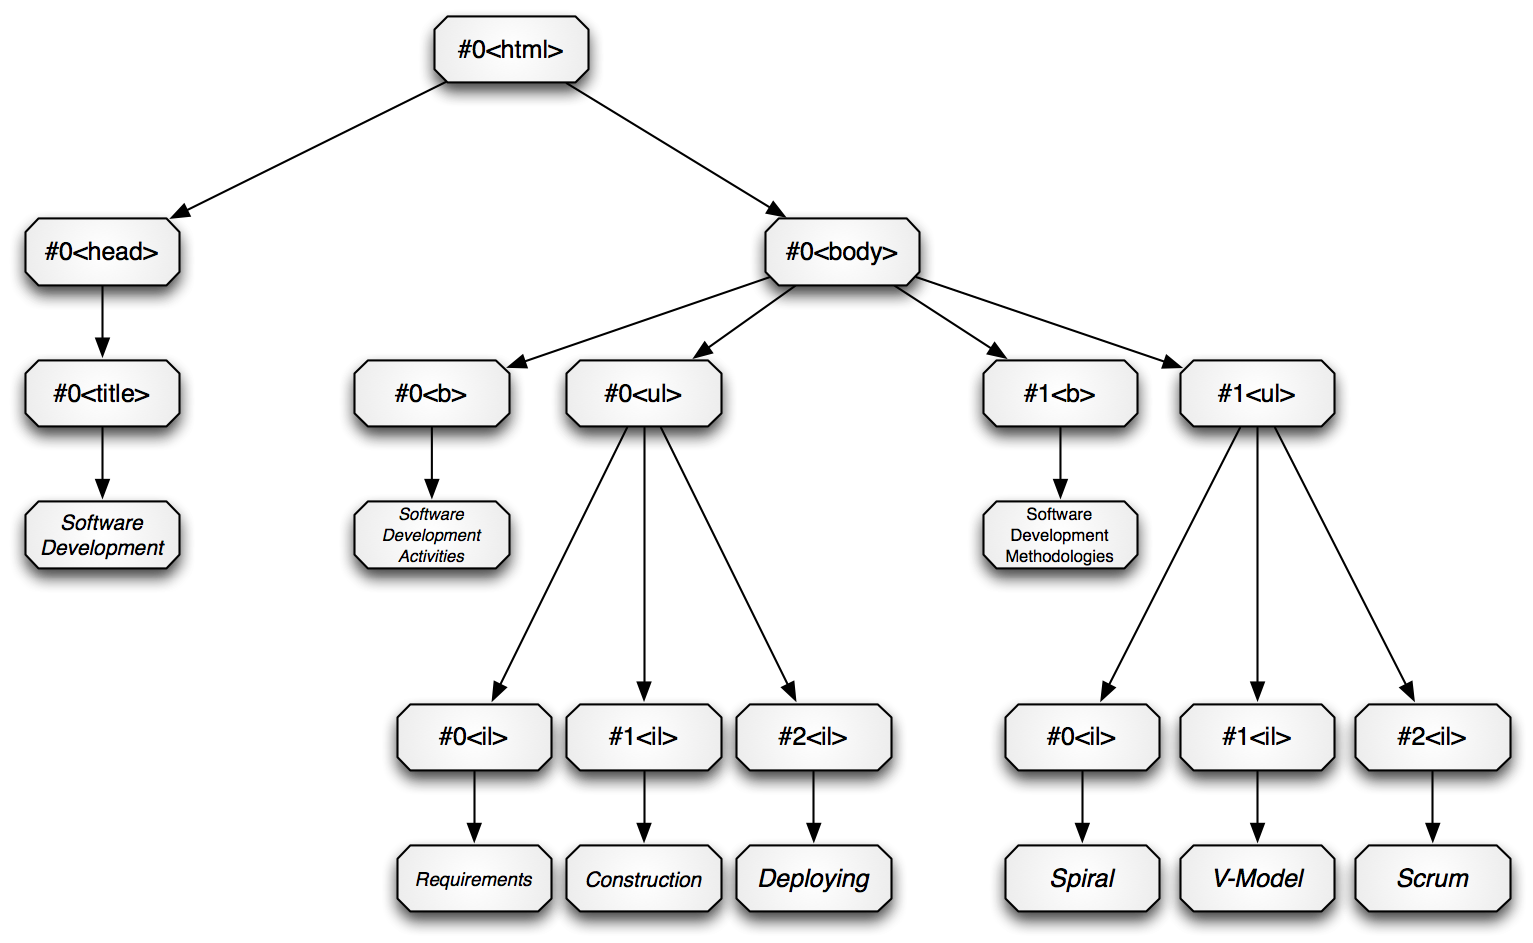
\includegraphics[width=13cm]{images/dom-paramaterized-tree-example.png}
		\caption{Example for parameterized DOM tree}
		\label{dom-paramaterized-tree-example}
\end{figure} 
